\documentclass[a4paper,10pt]{article}

\usepackage[utf8]{inputenc}
%\usepackage[T1]{fontenc}

\usepackage{textcomp}           % Extra Symbole (Grad Celsius etc.)
\usepackage{amssymb,amsmath}    % Schöne Formeln (AMS = American Mathematical Society)
\usepackage{graphicx}           % Bilder und Seitenränder
\usepackage{subcaption}			% captions for subfigures
\usepackage{booktabs}           % Schönere Tabellen
\usepackage{colortbl}           % Farbige Tabellen

%\usepackage{tcolorbox}			% schöne bunte Boxen
\usepackage{mathtools}			% \mathclap für ordentliche \underbrace-			environments
\usepackage[left=2cm,right=2cm,top=2cm,bottom=2cm]{geometry}			% Pagelayout mit \newgeometry, \restoregeometry
\usepackage{float}
\usepackage{wrapfig}
\usepackage{enumitem}
\usepackage{float}
\usepackage{braket}
\usepackage{caption}
\usepackage{verbatim}
\usepackage[per-mode=reciprocal,output-decimal-marker={.},binary-units=true,separate-uncertainty=true]{siunitx}
\usepackage[breaklinks=true,colorlinks=true,linkcolor=blue,urlcolor=blue,citecolor=blue]{hyperref}
\usepackage{physics}
\usepackage{url}
\usepackage{subcaption}
\usepackage{calrsfs}
\usepackage{tikz}
\usetikzlibrary{decorations, positioning, intersections, calc, shapes,arrows, scopes}
\DeclareMathAlphabet{\pazocal}{OMS}{zplm}{m}{n}

\graphicspath{{./img/}}

\newcommand{\dif}{\mathrm{d}}

\bibliographystyle{instant}

\renewcommand{\k}{\mathbf{k}}
\begin{document}
\begin{titlepage}
 \begin{center}
	\Large{Advanced laboratory class 3}
	\end{center}
	\begin{center}
	 \LARGE{\textbf{FP3 - Supersonic Gas Expansion}}
	\end{center}

	\begin{center}

	\large Marco \textsc{Canteri} \\
	marco.canteri@student.uibk.ac.at\\
	\large Maximilian \textsc{Münst} \\
	maximilian.muenst@student.uibk.ac.at
	\end{center}

	\begin{center}
	\vspace{1cm}
	Innsbruck, \today
	\vspace{1cm}
	\end{center}

	\begin{abstract}

  \end{abstract}
  \vspace{1cm}

	\begin{center}
	
\includegraphics[scale=0.4]{img/uibk}
	\end{center}

\end{titlepage}

\section{Introduction}
Supersonic expansion of an atomic or molecular gas is a means often used in chemical or ion physics. For example it is used to perform spectroscopy \cite{demtroeder} or to analyse the pressure ionization behaviour  of a gas as it is done in this experiment. Furthermore, the low temperatures reached by supersonic expansion also allows for the growth of clusters, so there is also applications in cluster physics.

\section{Theoretical Background}
% I think we should expand this section whenever we use something in the analysis.
The theory presented in this section is based on the book "Gase, Nanosysteme, Flüssigkeiten".\cite{bergmann}

\subsection{Knudsen Number}
The Knudsen Number describes the ratio of the mean free path length $l$ of a particle and the characteristic length of the containing vessel $L$.
\begin{equation}
  K_n = \frac{l}{\sqrt{2} L} = \frac{k_B T }{\sqrt{2} \pi d^2 p L}
\end{equation}
Here, the last term can be applied to Boltzmann gases. $T$ is the temperature, $d$ is the radius of the hard sphere potential of the Argon atoms, $p$ is the pressure inside the vessel and $k_B$ is the Boltzmann constant.

\subsection{Velocity Distribution}
In the two final parts a look is taken at the distribution of velocities of particles in a gas pulse. According to \cite{bergmann}, the velocity in the gas pulse follows the floating Maxwellian distribution 
\begin{equation}
	f(v) = C v^2 \exp(- \frac{m (v - u)^2}{2 k_\mathrm{B} T}) = C v^2 \exp(\mathrm{S}_\parallel (1 - \frac{v}{u})^2),
\end{equation}
where $\mathrm{S}_\parallel = \sqrt{\frac{1}{2} m u^2 / (k_{\mathrm{B}} T_\parallel)}$ is the parallel speed ratio and $u$ or is the maximum drift velocity of the gas pulse. Finally $C$ is a normalization factor. The longitudinal temperature can be calculated as 
\begin{equation}
	T_\parallel = \frac{m}{2 k_\mathrm{B}} \big(\frac{u}{\mathrm{S}_\parallel} \big)^2.
\end{equation}

\section{Experimental Setup}
The experiment consists of a two main chambers. In the first one the input gas (i.e. Argon and later Helium) is contained. The pressure in the first chamber is not constant but is at a magnitude of a few \si{\bar} throughout the experiment. The second chamber is continuously emptied by a turbo-molecular pump, which is backed by a diaphragm pump. The chambers are connected via an orifice that is opened and closed by a piezo crystal. To vary the frequency and the time period of inlet one just has to accordingly modulate the electrical pulses on the piezo.
\newline
The open orifice allows for a small gas pulse to reach the vacuum chamber, where it can expand first with supersonic speed, which is followed by effusive expansion. This leads to a change in the measured pressure inside the vacuum chamber, which is measured by a cold cathode ionization gauge.\cite{cold_cathode} To put it into simple terms, a DC voltage excites a discharge between to unheated electrodes (cathode and anode). Positive and negative charge carriers produced by collisions of electrons and gas particles move to their respective electrode and are detected. However, to properly use this method, one has to include a correction for the used gas, as different gases have different ionization behaviour.
\\
The output from the ionization gauge is technically speaking a voltage, which is measured with an oscilloscope. To convert the voltage into pressure a formula given in the data sheet \cite{datasheet_pfeiffer} is used. 
\begin{equation}
	\label{eq_pressure}
	p = K \exp(1.667 \times U - 9.333)
\end{equation}
Here, $U$ indicates the voltage signal that the gouge generates, while $K$ is a proportionality factor that corrects for the gas in use. The data sheet gives $K= 0.8$ for argon and $K = 5.9$ for helium. Eq. \ref{eq_pressure} takes the voltage in \si{\volt}, the resulting pressure is given in \si{\pascal}.
\\
While the pressure is measured at the top of the setup, a more interesting part is happening in the center. The pulse travels through two ring-shaped electrodes that are charged with a DC voltage. When there is enough gas in between the electrodes a plasma discharge is caused. This leaves both ionized and excited argon atoms in the pulse which can subsequently by detected with a channeltron detector.
\\
The channeltron is connected to a oscilloscope to visualize the measured data. Furthermore, the output of the ionization gauge and the voltage on the resistor on the electrode are fed into the oscilloscope.
\begin{figure}[H]
    \centering
    \tikzstyle{chamber2} = [draw, rectangle,
    minimum height=10em, minimum width=20em]
    \tikzstyle{chamber1} = [draw, rectangle, minimum height = 10em, minimum width = 5em]
    \tikzstyle{coldcathode} = [draw, rectangle, minimum height = 2em, minimum width = 2em]
    \tikzstyle{electrode} = [draw, ellipse, minimum height = 5em, minimum width = 2em]
    \tikzstyle{channeltron} = [draw, rectangle, minimum height = 5em, minimum width = 1em]
    \tikzstyle{orifice} = [draw, rectangle, fill=black!100, minimum height = 0.5em, minimum width = 0.5em]
    \tikzstyle{resistor} = [draw, rectangle, minimum height = 1em, minimum width = 2em]
    \tikzstyle{sum} = [draw, fill=blue!20, circle, node distance=1cm]
    \tikzstyle{input} = [coordinate]
    \tikzstyle{output} = [coordinate]
    \tikzstyle{pinstyle} = [pin edge={to-,thin,black}]

\begin{tikzpicture}[auto, node distance=2cm,>=latex']
  \node at (0, 0) [chamber2, name = vacuum] {};
  \node at (-12.5em, 0) [chamber1, name = pressured] {};
  \node at (0, 6em) [coldcathode, name = pressuremeter] {};
  \node at (10.5em, 0) [channeltron, name = channeltron] {};
  \node at (0, 0) [electrode, name = electrode1] {};
  \node at (4em, 0) [electrode, name = electrode2] {};
  \node at (-10em, 0) [orifice, name = orifice] {};
  \node at (-6em, -7em) [resistor, name = resistor] {};
  \node at (-9em, -7em) [name = voltage] {$V$};
  \node at (7.5em, 7em) [name = deflect] {$V_\mathrm{Deflect}$};

  \draw  (electrode1) |- (resistor);
  \draw (resistor) -- (voltage);
  \draw (electrode2) -- (4em, -7em);
  \draw (3.5em, -7em) -- node[below] {GND} (4.5em, -7em);
  \draw (6.5em, 2.5em) -- node[below] {} (8.5em, 2.5em);
  \draw (7.5em, 2.5em) -- (deflect);

  \node at (-6em, -8em) {$R$};
  \node at (14em, 0) {Channeltron};
  \node at (0, 8em) {Ionization gauge};
  \node[text width = 3cm,align = center] at (-12.5em, -4em) {Pressure \\ chamber};
  \node at (0, -4.5em) {Vacuum chamber};
  \node at (-8em, 1em) {Orifice};
\end{tikzpicture}
\caption{Sketch of the experimental setup. Gas passes from the pressure chamber into the vacuum chamber in pulses, where the length and the frequency can be varied. The pressure is measured with the cold cathode ionization gauge. A direct voltage can be applied to the two ring electrodes, which causes a plasma discharge when gas is passing through. The discharge can be made visible by measuring the voltage on the resistor $R$. Finally the Channeltron detector can measure the intensity of atoms excited by the plasma discharge. }
\label{fig_setup}
\end{figure}
In this experiment one is mostly interested in the intensity of the excited argon atoms which makes the ionized argon atoms a unwanted interference in the detector's signal. Therefore the setup also has a deflection shield to divert the ionized argon atoms. However, in the experiment we found that tuning the deflection voltage did not notably increase the quality of the received signal.

\section{Procedure and Analysis}
\subsection{Pressure Characteristics}
Starting off, a look was taken at the pressure characteristics of the setup. To be specific, the pressure in the vacuum chamber was measured depending on the frequency and the width of the opening pulse. Measurements were performed on opening time windows with length \SI{120}{\micro \s}, \SI{190}{\micro \s} and \SI{230}{\micro \s} at frequencies of \SI{1}{\hertz}, \SI{2}{\hertz}, \SI{5}{\hertz} and \SI{10}{\hertz}. To measure the pressure in the pressure chamber a manometer on the inlet pipe was used. The indicated pressure of did not notably change throughout this part of the experiment, which leaves a pressure of \SI{2.9(1)}{\bar}. The results are plotted in Fig. \ref{fig_pressure_characterization} and Fig. \ref{fig_width_characterization}. Both figures show the same data, but in Fig. \ref{fig_pressure_characterization} the data is grouped according to frequency and in Fig. \ref{fig_width_characterization} it is arranged according to pulse width. As one can see in Fig. \ref{fig_pressure_characterization} the length of the pulse positively correlates with height of the pressure peak, i.e. the longer the pulse the higher the peak, which one would expect. However, the values of the ratio of the peak heights is clearly different than the ratio of the pulse length, which would be $1:1.56:1.92$. The ratio of the measured peaks however is approximately $1:40:69$. As the ratio between the second and the third number seems to be way closer to the ratio of the respective pulse widths it is probable that there is a time delay on the opening of the nuzzle, which causes less gas to pass then one would expect. Additionally, it would also explain why the difference shrinks with increasing opening time. 


\begin{figure}[H]
  \centering{}
  \begin{subfigure}[t]{0.45 \textwidth}
    \centering
    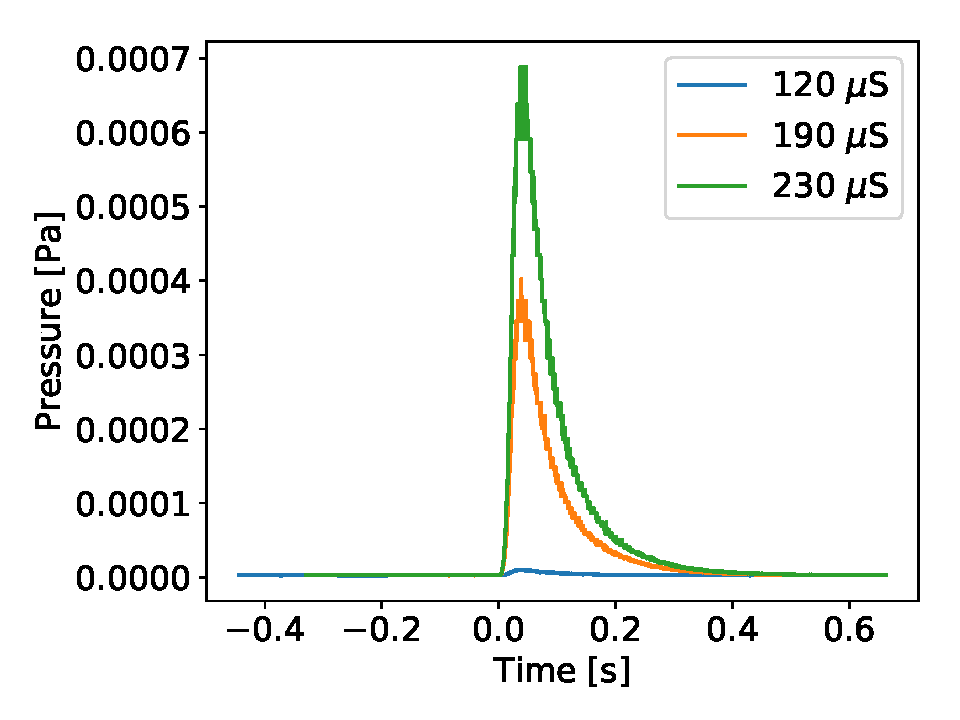
\includegraphics[height=6cm]{part1_1_hertz.pdf}
    \caption{\SI{1}{\hertz}}
  \end{subfigure}
  ~
  \begin{subfigure}[t]{0.45 \textwidth}
    \centering
    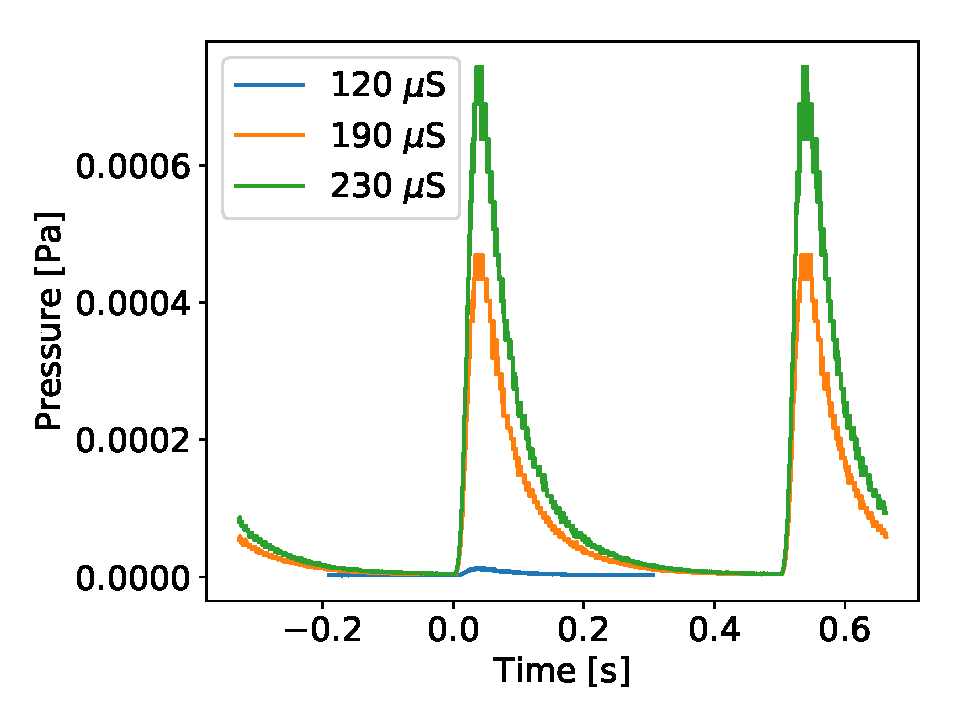
\includegraphics[height=6cm]{part1_2_hertz.pdf}
    \caption{\SI{2}{\hertz}}
  \end{subfigure}
  ~
  \begin{subfigure}[t]{0.45 \textwidth}
    \centering
    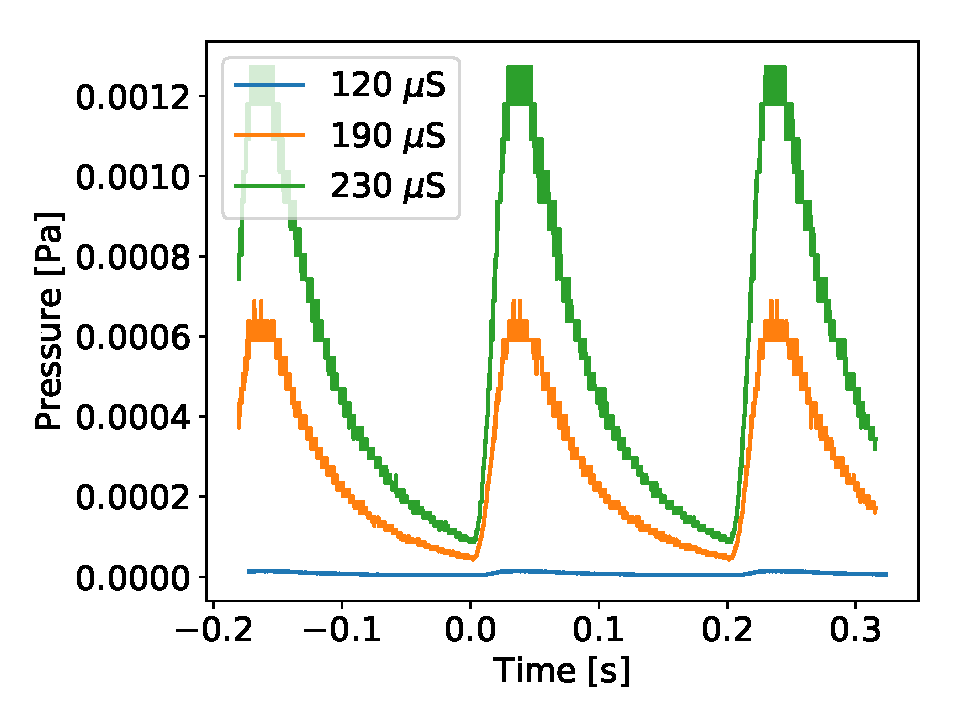
\includegraphics[height=6cm]{part1_5_hertz.pdf}
    \caption{\SI{5}{\hertz}}
  \end{subfigure}
  ~
  \begin{subfigure}[t]{0.45 \textwidth}
    \centering
    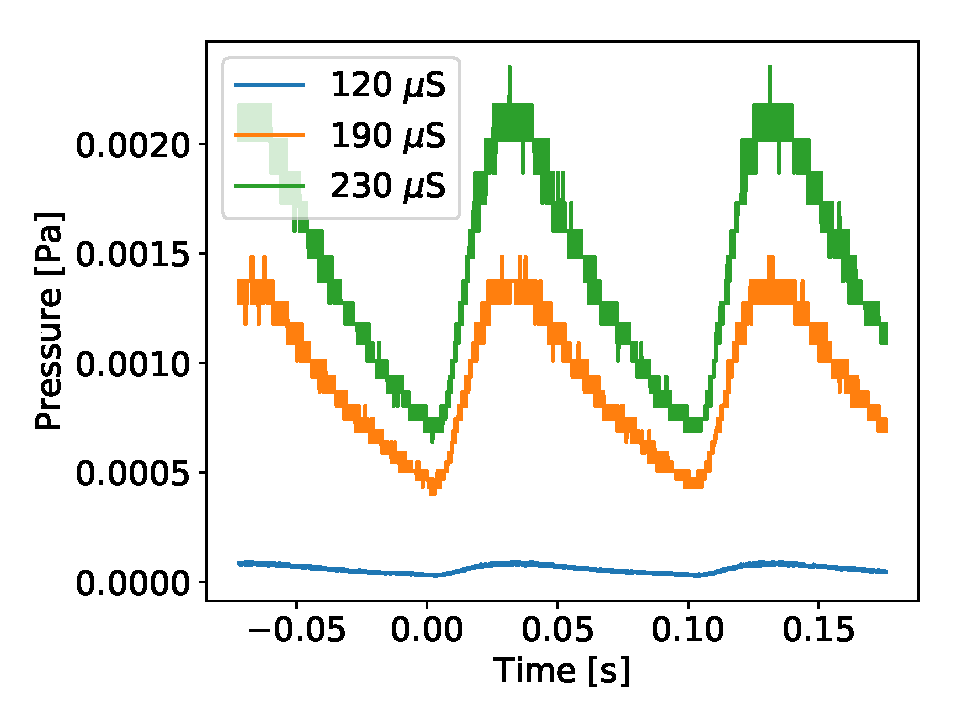
\includegraphics[height=6cm]{part1_10_hertz.pdf}
    \caption{\SI{10}{\hertz}}
  \end{subfigure}
  \caption{Depiction of the measured pressure for pulse widths of \SI{120}{\micro \s}, \SI{190}{\micro \s} and \SI{230}{\micro \s} at the displayed frequency. }
  \label{fig_pressure_characterization}
\end{figure}
Fig. \ref{fig_width_characterization} shows the same curves, but now curves with the same opening time are grouped up. The first thing one notices is that the higher the frequency is, the higher is the maximum value of the pressure curve. This one would expect because the vacuum pump can simply not sufficiently evacuate the vacuum chamber between the pulses as one can see for the \SI{5}{\hertz} and \SI{10}{\hertz} curves, meaning that there is additionally to the pulse a background pressure, which leads to a higher maximum. 
\\
However, one furthermore sees that the difference in the minimum to maximum pressure value also depends on the frequency. This is unexpected, as the opening width is the same in every plot in Fig. \ref{fig_width_characterization}. Apparently there is a systematic error that is connected to the frequency and the time width of the opening. %It was already mentioned that there is likely a delay in the opening. 
\\
In Fig. \ref{fig_pressure_characterization} and Fig. \ref{fig_width_characterization} we saw that both the frequency and the opening width influence the pressure span between minimum and maximum. Our idea to explain this is the following: In the script \cite{script} it says that the piezo closes the nozzle by pressing a rubber joint on the opening of the nozzle. It might be that the rubber joint sticks to nozzle, which would explain why there is a slight delay on the opening time. Furthermore, it is possible that the rubber sticks tighter to the nozzle the longer it is pressed to it by the piezo. This would then also explain why the inlet of gas is higher the higher the frequency is. 

% Maybe we should take a look at the behaviour of maximum pressure and decay time \tau depending on frequency/width?
\begin{figure}[H]
  \centering{}
  \begin{subfigure}[t]{0.45 \textwidth}
    \centering
    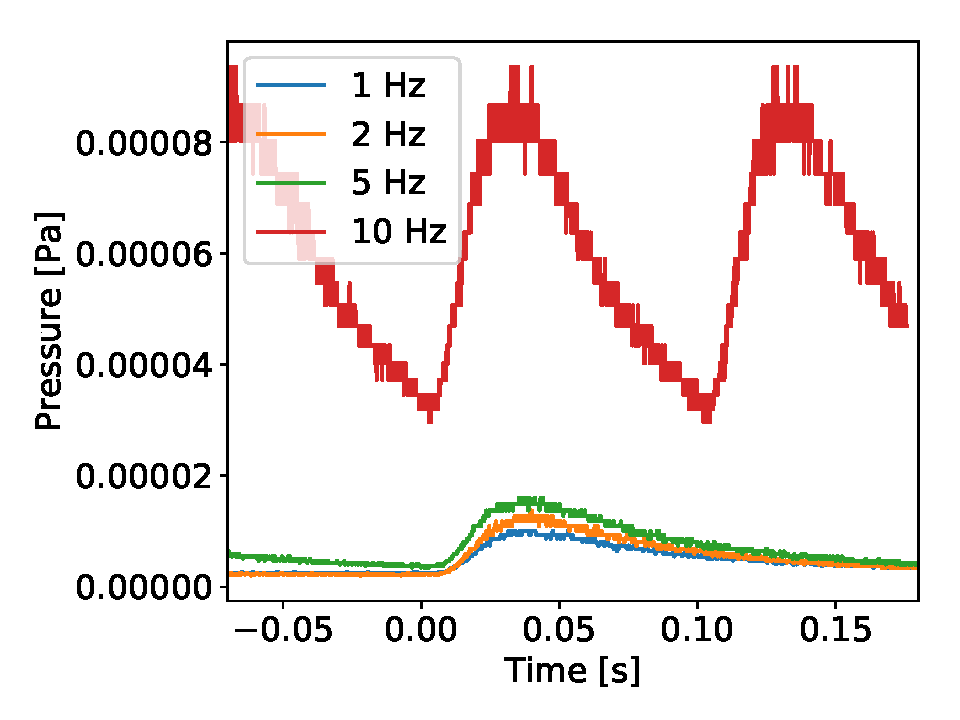
\includegraphics[height=6cm]{part1_120_width.pdf}
    \caption{\SI{120}{\micro \s}}
  \end{subfigure}
  ~
  \begin{subfigure}[t]{0.45 \textwidth}
    \centering
    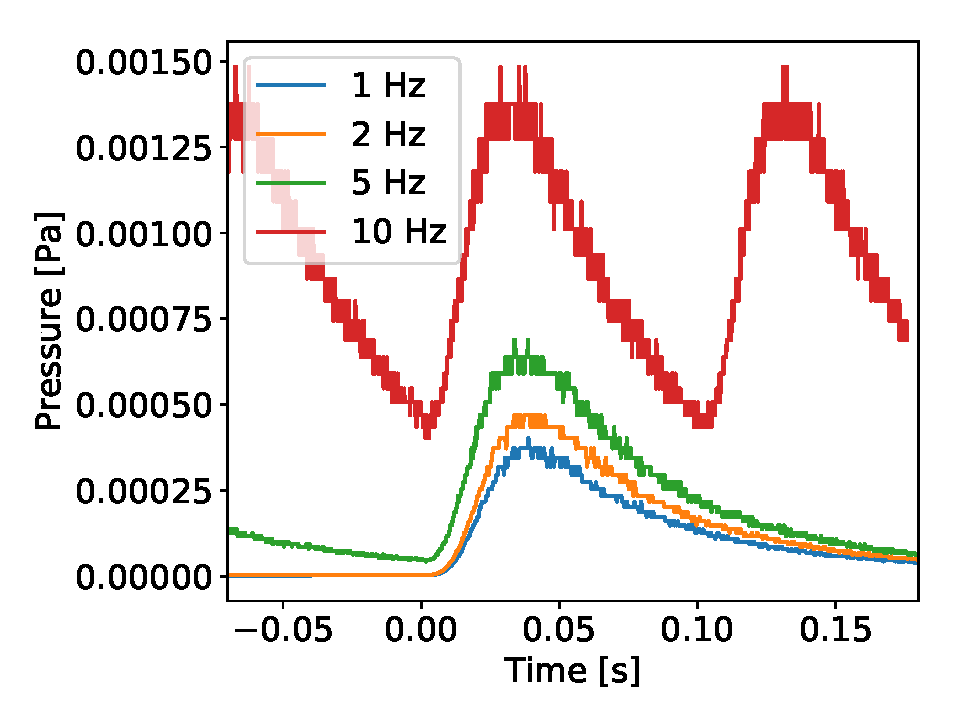
\includegraphics[height=6cm]{part1_190_width.pdf}
    \caption{\SI{190}{\micro \s}}
  \end{subfigure}
  ~
  \begin{subfigure}[t]{0.45 \textwidth}
    \centering
    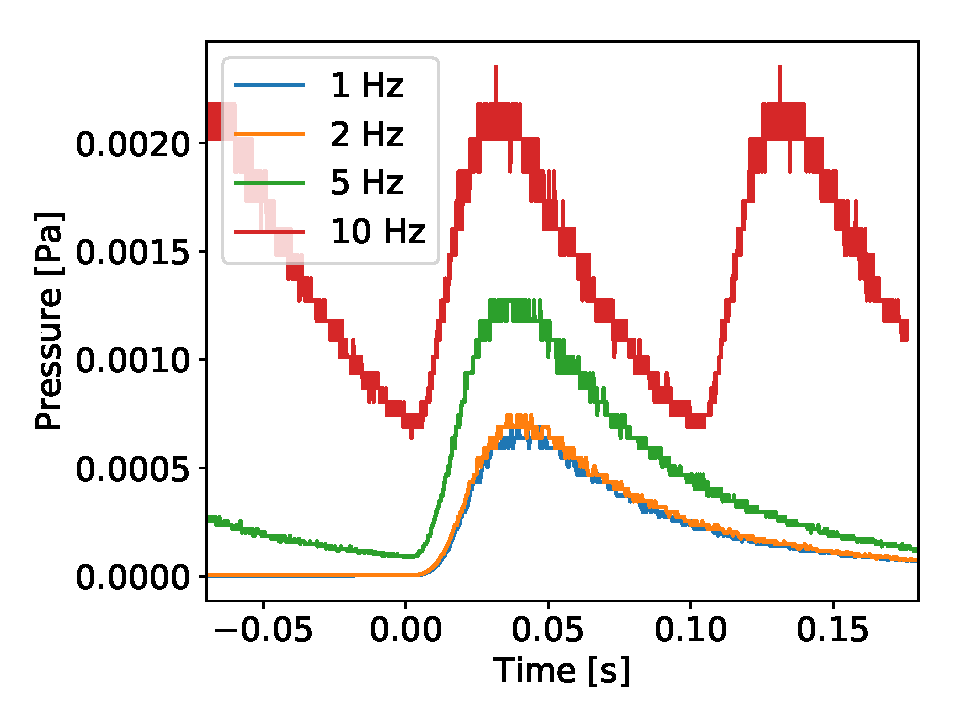
\includegraphics[height=6cm]{part1_230_width.pdf}
    \caption{\SI{230}{\micro \s}}
  \end{subfigure}
  \caption{Plots of the pressure behaviour with variable frequency and fixed opening time. The data is the same as in Fig. \ref{fig_pressure_characterization}, but arranged with respect to pulse width instead of frequency. }
  \label{fig_width_characterization}
\end{figure}

\subsection{Gas Inlet per Pulse}
To calculate how much gas gets into the vacuum chamber every time the nuzzle is opened, we have to first determine the Knudsen number. If $K_n \gg 1$ then there is hardly any collisions between atoms, meaning that the energy distribution on various inner degrees of freedom should be conserved and therefore the temperature should not change. However, if the Knudsen number is small, then we should see an adiabatic expansion, which of course includes a change in temperature. This consideration is relevant because we have to use different formulas for the calculation of the inlet if the Knudsen number is big or small. 
\\
As Fig. \ref{fig_knudsennumber} shows, the Knudsen number is very high during the pulse. As one would expect, it reaches its minimum when the pressure peaks, but even so the value is still $56$. % we must use the precise value with error, I just approximated it with the graph
This means that we are not in the adiabatic regime and must therefore use the equation 
\begin{equation}
	\frac{P_i}{V_i} = \frac{P_f}{V_f},
\end{equation}
where $P_i$ and $V_i$ are the initial pressure and initial volume inside the nozzle, while $P_f$ and $V_f$ are the final pressure and volume. We measured $P_i$ and we used $4\pm 1$ L for $V_f$ which is approximately the volume of the vacuum chamber. $P_f$ is extracted from the data as the value of the peak. Therefore is possible to find $V_i$ which is the gas inlet. In the following table the results can be found
\begin{table}[H]
\centering
\begin{tabular}{ccc} \toprule
    Gas inlet [mL] & Opening time [$\mu$s] & Frequency \\ \midrule
$1.3931\cdot 10^{-7} \pm 3\cdot 10^{-11}$& 120& 1\\
$5.549\cdot 10^{-6} \pm 1\cdot 10^{-9}$& 190& 1\\
$9.499\cdot 10^{-6} \pm 2\cdot 10^{-9}$& 230& 1\\\midrule
$1.8937\cdot 10^{-7} \pm 5\cdot 10^{-11}$& 120& 2\\
$6.471\cdot 10^{-6} \pm 2\cdot 10^{-9}$& 190& 2\\
$1.0256\cdot 10^{-5} \pm 2\cdot 10^{-9}$& 230& 2\\ \midrule
$2.2080\cdot 10^{-7} \pm 5\cdot 10^{-11}$& 120& 5\\
$9.499\cdot 10^{-6} \pm 2\cdot 10^{-9}$ & 190& 5\\ 
$1.7554\cdot 10^{-5} \pm 4\cdot 10^{-9}$ & 230& 5\\\midrule
$1.2907\cdot 10^{-6} \pm 3\cdot 10^{-10}$& 120& 10\\ 
$2.0467\cdot 10^{-5} \pm 5\cdot 10^{-9}$ & 190& 10\\
$3.2442\cdot 10^{-5} \pm 8\cdot 10^{-9}$ & 230& 10\\ \bottomrule
\end{tabular}
\caption{Gas inlet for various opening time and frequency. }
\end{table}

\begin{figure}[H]
	\centering
	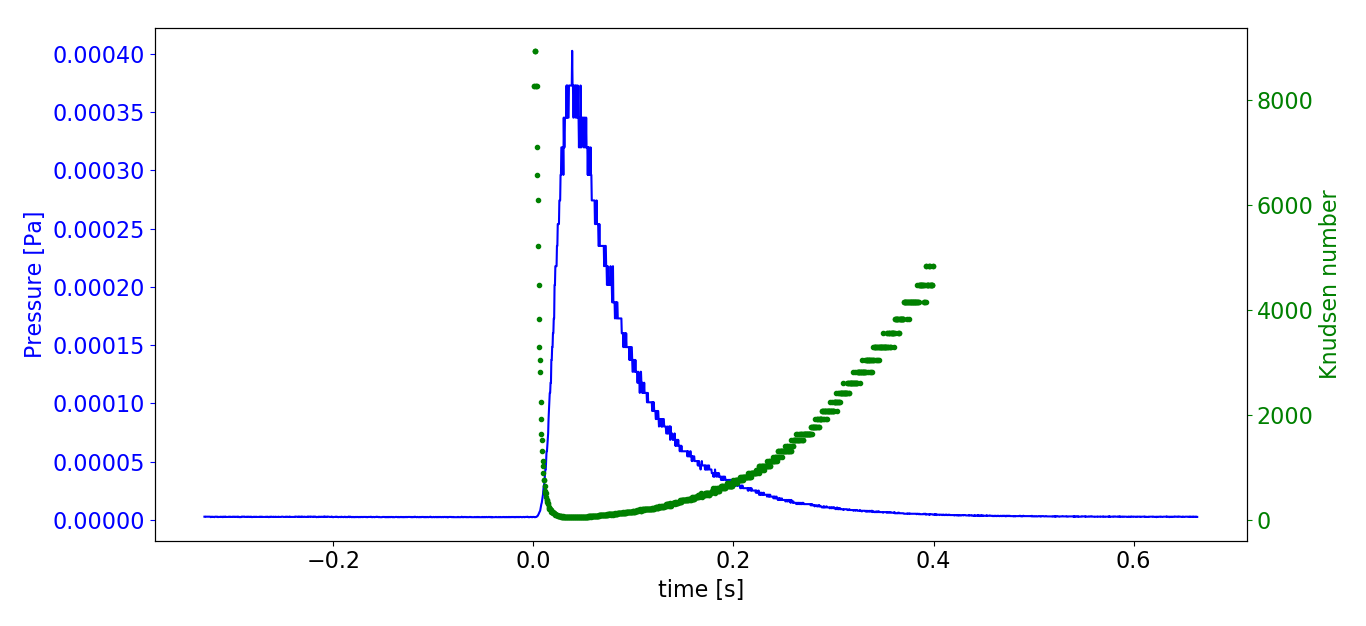
\includegraphics[width = \textwidth]{knudsen}
	\caption{Depiction of the behaviour of the Knudsen number during a pulse. Even though the number decreases during the pulse, it never comes close to zero but reaches its minimum at $56$. }
	\label{fig_knudsennumber}
\end{figure}

\subsection{Pressure drop}
After the gas pulse the pressure drop due to the gas been sucked up by the vacuum pump, we studied this drop by fitting an exponential decay of the form
\[f(t) = Ae^{-(t - t_0)/\tau} + C,\]
where $\tau$ is the parameter that gives the time scale of the decay, which we are interested in. All other parameters are not important in the analysis. An example of fit can be seen in figure \ref{expfit}. Below a table with the time scale $\tau$ for every measurement we took
\begin{table}[H]
\centering
\begin{tabular}{ccc} \toprule
    time scale $\tau$ [s] & Opening time [$\mu$s] & Frequency \\ \midrule
$0.07028 \pm 0.0005 $& 120& 1\\
$0.0575 \pm 0.0002$& 190& 1\\

$0.0567 \pm 0.0002$& 230& 1\\\midrule
$0.0639 \pm 0.0004$& 120& 2\\
$0.0590 \pm 0.0005$& 190& 2\\
$0.0556 \pm 0.0002 $& 230& 2\\ \midrule
$0.116 \pm 0.008$& 120& 5\\
$0.089 \pm 0.004$ & 190& 5\\ 
$0.110 \pm  0.006$ & 230& 5\\\midrule
$0.17 \pm  0.02$& 120& 10\\ 
$0.19 \pm 0.03$ & 190& 10\\
$0.28 \pm 0.05 $ & 230& 10\\ \bottomrule
\end{tabular}
\caption{Time scale for various opening time and frequency. }
\end{table}

From the data we can notice that the time scale is larger for bigger frequency and it seems it does not depend on the opening time. It is interesting to see the dependence of the time scale with the gas inlet calculated in the previous section. This is plotted in figure \ref{gasinlettimescale}, but as we can see there is apparently no correlation between the two quantities.

\begin{figure}[H]
\centering
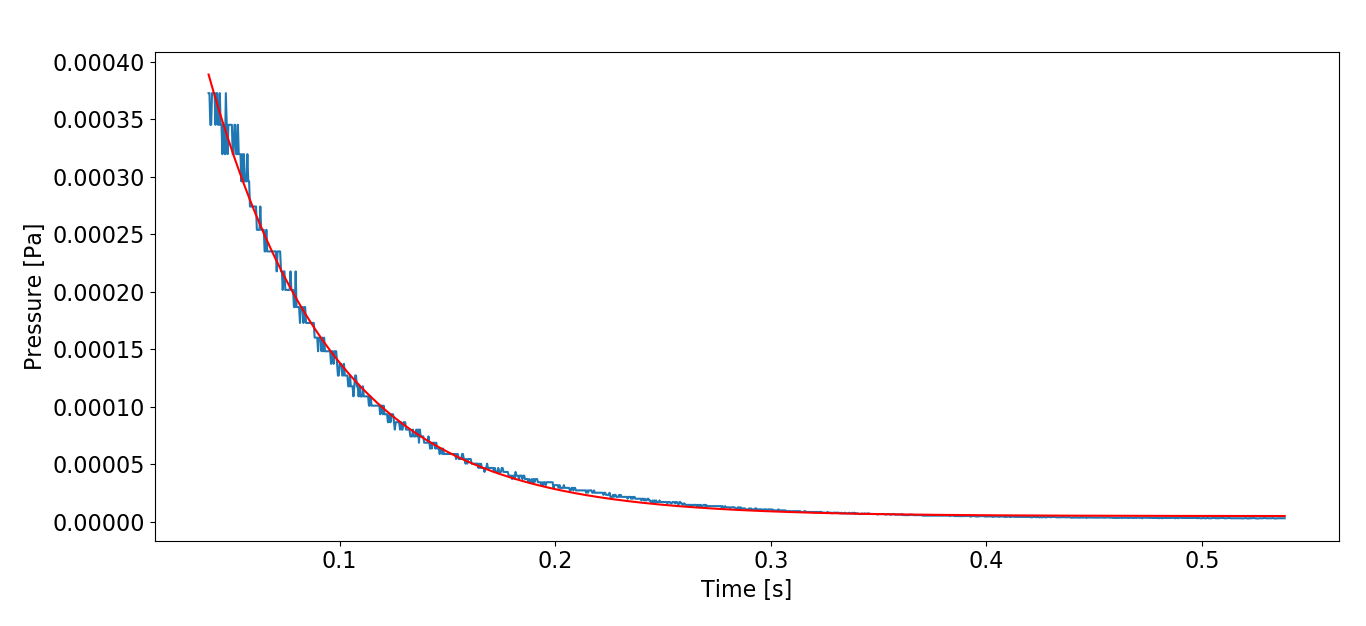
\includegraphics[width = 0.8\textwidth]{expfit}
\caption{Exponential fit for the measurement taken with opening time of 190 $\mu S$ and 1 Hz frequency.}\label{expfit}
\end{figure}

\begin{figure}[H]
\centering
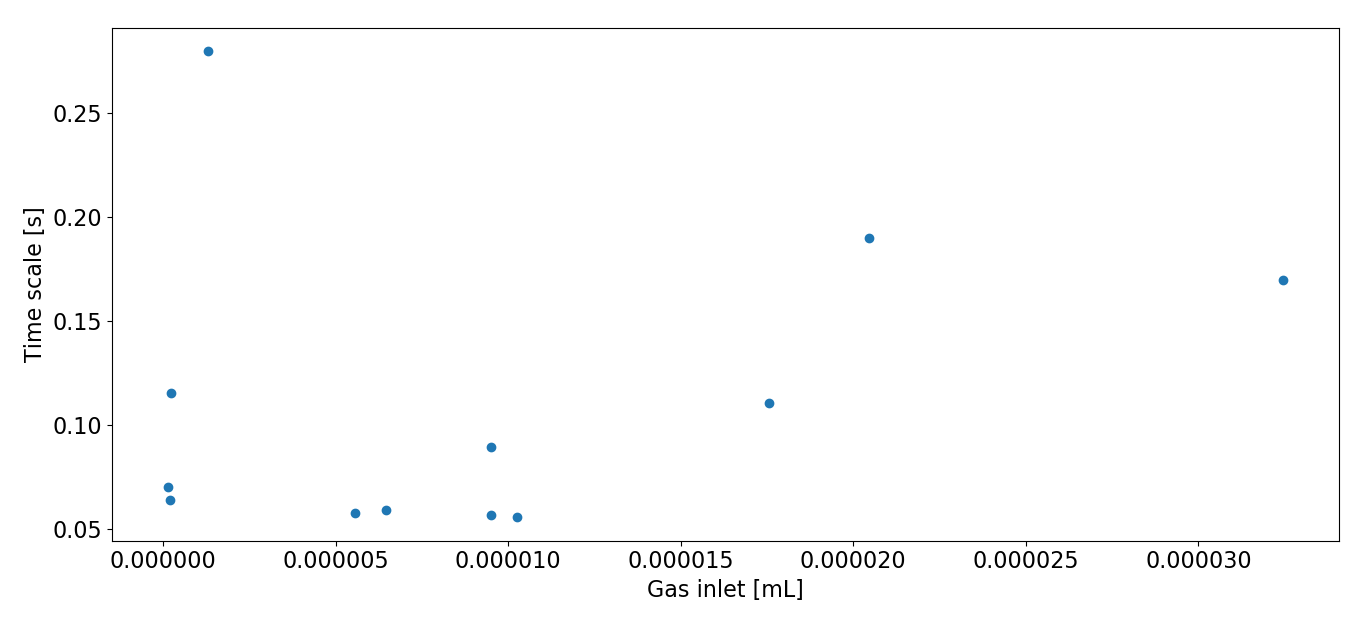
\includegraphics[width = 0.8\textwidth]{gasinlettimescale}
\caption{Time scale $\tau$ as a function of the gas quantity of the beam.}\label{gasinlettimescale}
\end{figure}

\subsection{Plasma discharge}
After studying the gas pulse, we tried to produce a plasma discharge. A power supply with a voltage of around 1000 V was attached to two rings electrodes as described in the experiment setup section. We fixed the opening time and frequency of the nozzle to 230 $\mu$s and 10 Hz. Then we tried to hit the gas at the right moment with a voltage pulse to produce a plasma discharge, this was done varying the delay of the electric pulse. We took three measurements for three different widths of the pulse, which can be seen in figure \ref{discharge}. 

\begin{figure}[H]
\centering
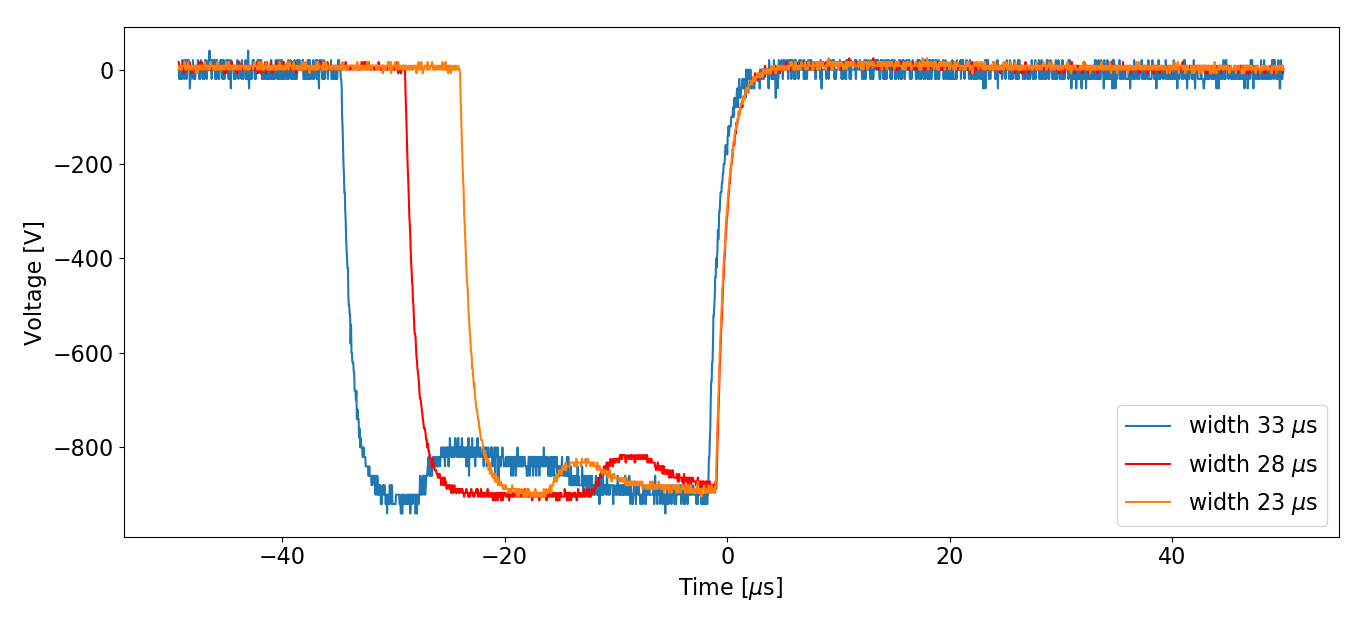
\includegraphics[width = \textwidth]{discharge}
\caption{Voltage on the electrodes, the delay of the pulse was modified every time to hit the gas pulse.}\label{discharge}
\end{figure}

We can clearly see the plasma discharge by the characteristic bump in the voltage during the pulse. This means that we are able to hit the gas pulse and induce a plasma discharge in the gas.

\subsection{Channeltron characterization}
Before starting the real measurement, we had to characterize the detector. We tried to apply different voltage on the channeltron and analysed its signal. In figures \ref{channeltron}
we can see the measurements. 
\begin{figure}[H]
  \centering{}
  \begin{subfigure}[t]{0.45 \textwidth}
    \centering
    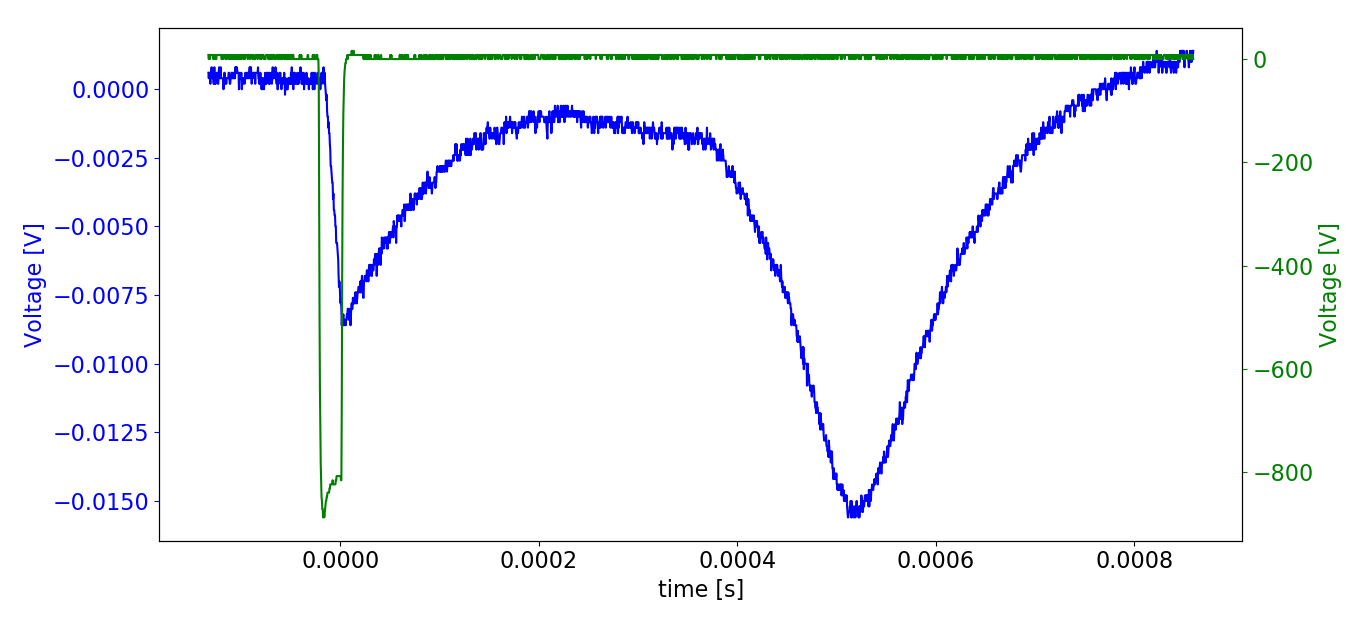
\includegraphics[width= \textwidth]{channeltron1}
    \caption{Channeltron voltage -1008 V}\label{channeltron1}
  \end{subfigure}
  ~
  \begin{subfigure}[t]{0.45 \textwidth}
    \centering
    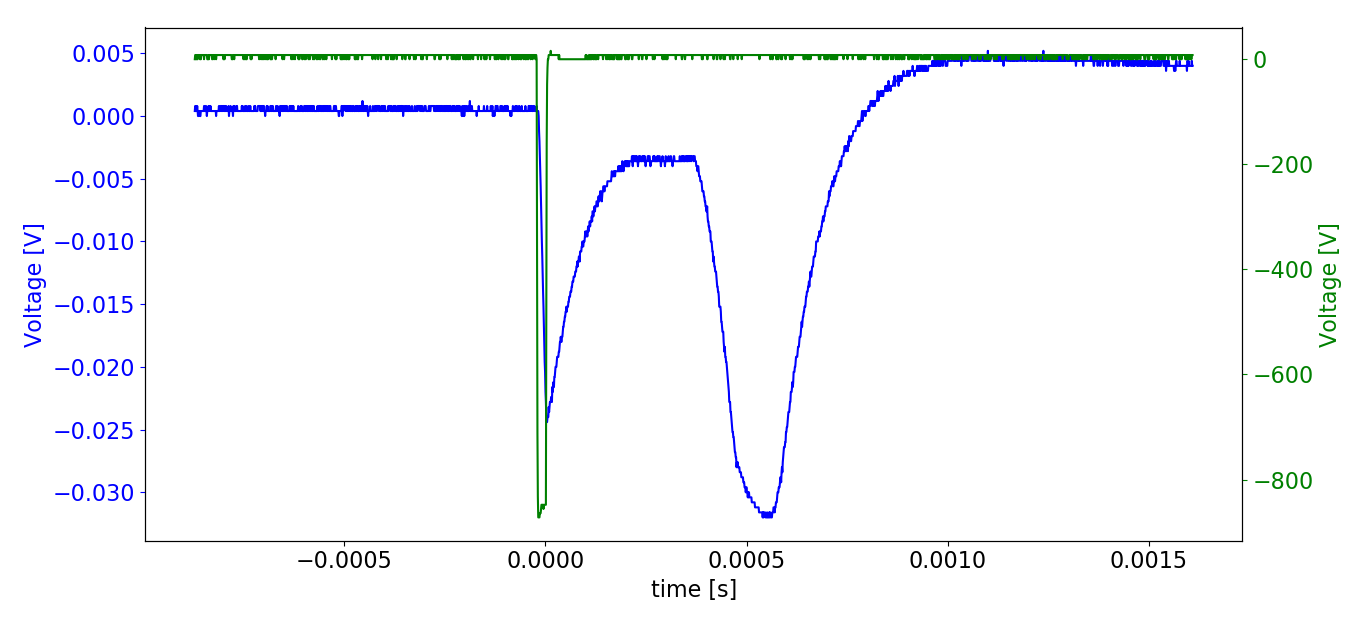
\includegraphics[width=\textwidth]{channeltron2}
    \caption{Channeltron voltage -1105 V}\label{channeltron2}
  \end{subfigure}
  ~
  \begin{subfigure}[t]{0.45 \textwidth}
    \centering
    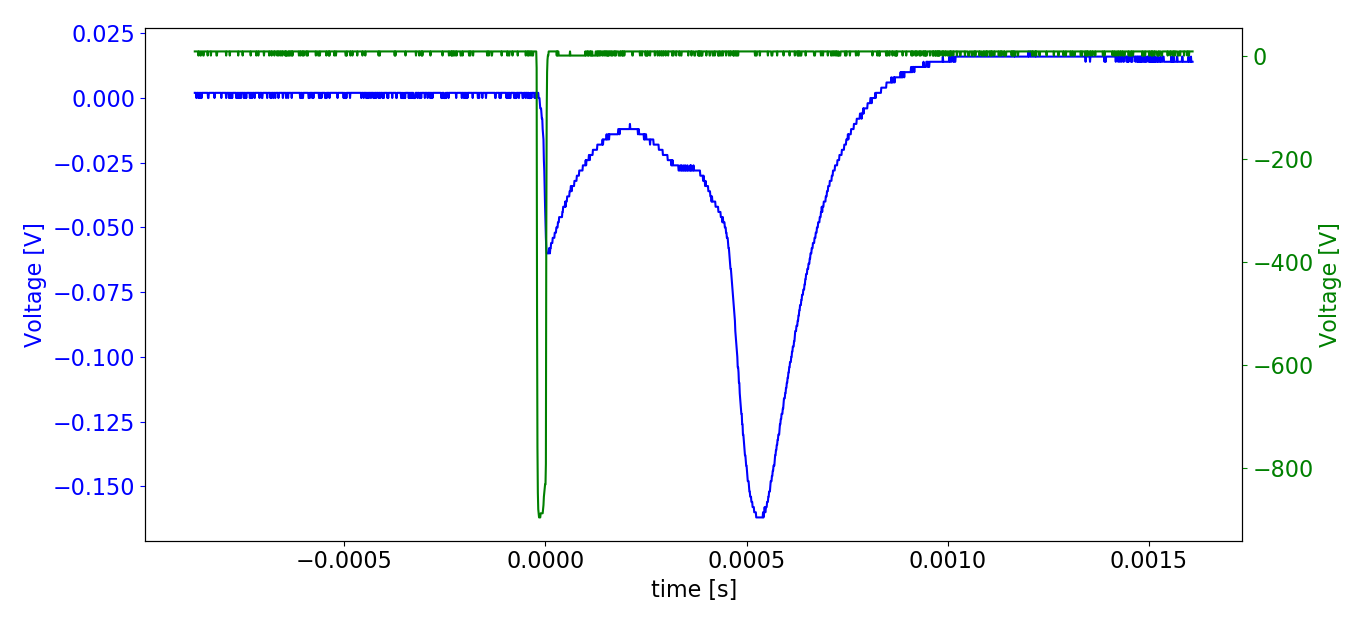
\includegraphics[width=\textwidth]{channeltron3}
    \caption{Channeltron voltage -1204 V}\label{channeltron3}
  \end{subfigure}
  ~
  \begin{subfigure}[t]{0.45 \textwidth}
    \centering
    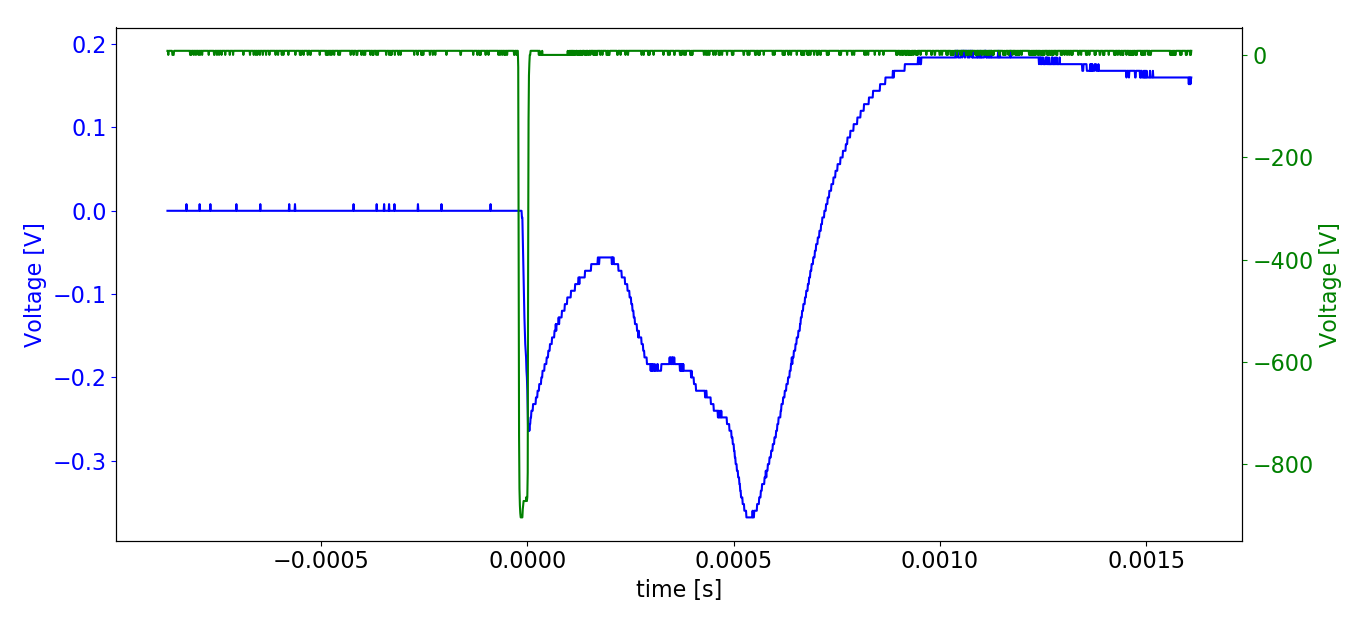
\includegraphics[width=\textwidth]{channeltron5}
    \caption{Channeltron voltage -1405 V}\label{channeltron4}
  \end{subfigure}
  \caption{Green line is the electric pulse for the plasma discharge. The blue line is the signal from the channeltron. All measurements were taken with a voltage on the deflector of -5 V. }
  \label{channeltron}
\end{figure}
In every plot we can clearly see at least two peaks, the fist peak is due to particles like electron and photons which are very fast, then after a while also the exited Argon arrives and gives the second large peak. In figure \ref{channeltron3} and \ref{channeltron4} a third peak between the two already described appears, it is very low, almost imperceptible, but it can be seen and it is due to ionized Argon, which is lighter then excited Argon and therefore faster. Furthermore, in all plots of figure \ref{channeltron} but the first one, an overshoot can be seen, after the last peak the voltage of the channeltron does not come back to the value before the measurement but it goes higher, we notice also that the overshoot is bigger for lower channeltron voltage. This helped us to choose the correct voltage to use for the channeltron, in fact we should reduce the overshoot as much as possible, but still be able to see all the peaks.  


\subsection{Argon lifetime and time of flight}
%Calculation of the velocity & Mach number
From the velocity one can now estimate the probability of an excited argon atom to decay before the detector is reached. This can be done with quite a simple integration:
\begin{equation}
	\mathbb{P} = \int_0^{t_F} \frac{1}{\tau} \exp(-\frac{t}{\tau}) \mathrm{d}t = 1 - \exp(-\frac{t_F}{\tau}) \approx 
\end{equation}
\subsection{Helium time of flight}

\section{Conclusion}

\begin{thebibliography}{99}
\bibitem{datasheet_pfeiffer}
\textsc{Pfeiffer Vakuum}, \textit{Compact FullRange Gauge -PKR 251 }, \url{http://www.idealvac.com/files/brochures/Pfeiffer_PKR_251_Pirani_ColdCathode.pdf}

\bibitem{demtroeder}
\textsc{W. Demtröder, H.-J. Foth}, \textit{Molekülspektren in kalten Düsenstrahlen}, \url{https://onlinelibrary.wiley.com/doi/pdf/10.1002/phbl.19870430104}

\bibitem{bergmann}
\textsc{Bergmann-Schäfer}, \textit{Gase, Nanosysteme, Flüssigkeiten}, \textit{Band 5} (de Gruyter, 2005)

\bibitem{cold_cathode}
\textsc{LDS Vacuum Shopper}, \textit{Cold Cathode Gauges}, \url{http://www.ldsvacuumshopper.com/cocaga.html}

\bibitem{script}
\textsc{Jennifer Meyer, Roland Wester}, \textit{Versuch im Fortgeschrittenen Praktikum FP3: Supersonische Düsenstrahlen}
\end{thebibliography}
\end{document}
